\subsection{Li\'enard System}
Consider the system
\begin{equation}{\label{eq:nols}}
	\begin{aligned}
		\dot{x}&=y-F(x)\\
		\dot{y}&=-g(x)
	\end{aligned}\quad\rightarrow\quad
	\ddot{x}+f(x)\dot{x}+g(x)=0\quad(f(x)=F^\prime(x))
\end{equation}
\begin{theorem}[\textbf{Li\'enard Theorem}]
	Suppose two functions $f(x)$ and $g(x)$ satisfy the following conditions
	\begin{itemize}
		\item $f(x)$ and $g(x)$ are continuously differentiable for all $x$
		\item $g(-x)=-g(x)\ \forall\ x$, i.e. $g(x)$ is an odd function
		\item $g(x)>0$ for $x>0$
		\item $f(-x)=f(x)\ \forall\ x$, i.e. $f(x)$ is an even function
		\item The odd function, $F(x)=\displaystyle\int_0^xf(u)du$, has exactly one positive zero at $x=\alpha$ (say), $F(x)$ is negative for $0<x<\alpha$, and $F(x)$ is positive and nondecreasing for $x>\alpha$ and $F(x)\rightarrow\infty$ as $x\rightarrow\infty$.
	\end{itemize}
	Then the Li\'enard equation \emph{(\ref{eq:nols})} has a \emph{\textbf{unique stable limit cycle}} surrounding the origin of the phase plane.
\end{theorem}
The Li\'enard system is a very special type of equation that has a unique stable
limit cycle.\\\\
Equation of Nonlinear Oscillators are given by introducing nonlinear terms in Equation (\ref{eq:tho})
\begin{equation}{\label{eq:nlo}}
	\ddot{x}+\gamma\dot{x}+\omega^2x+N(x,\dot{x})=0
\end{equation}
\subsection{Van-der-Pol Oscillator: $N(x,\dot{x}=x^2\dot{x})$}
The van-der-Pol oscillator is given by
\begin{equation}{\label{eq:vdpo}}
	\ddot{x}+\gamma\dot{x}+\omega^2x+\epsilon x^2\dot{x}=0\quad\rightarrow\quad
	\ddot{x}+\underbrace{(\gamma+\epsilon x^2)}_{\tilde{\gamma}}\dot{x}+\omega^2x=0
\end{equation}
Equation (\ref{eq:vdpo}) shows that for the van-der-Pol oscillator the damping ‘constant’ $\tilde{\gamma}$ becomes time dependent via the amplitude $x^2$.
\begin{itemize}
	\item $\gamma>0\quad\epsilon>0$\\ The effective damping $\tilde{\gamma}$ is always positive.
	The trajectories are evolving towards the origin, which is a stable fixed point.
	\item $\gamma<0\quad\epsilon<0$\\ The effective damping $\tilde{\gamma}$ is always negative.
	The system is unstable and the trajectories are evolving towards infinity.
	\item $\gamma>0\quad\epsilon<0$\\ For small values of the amplitude $x^2$ the effective damping $\tilde{\gamma}$ is positive leading to even smaller amplitudes.
	For large values of $x^2$ the effective damping $\tilde{\gamma}$ is negative leading a further increase in amplitude.
	The system evolves either towards the fixed point or towards infinity depending on the initial conditions.
	\item $\gamma<0\quad\epsilon>0$\\ For small values of the amplitude $x^2$ the effective damping $\tilde{\gamma}$ is negative leading to an increase in amplitude.
	For large values of $x^2$ the effective damping $\tilde{\gamma}$ is positive and the amplitude decreases.
	The system evolves towards a stable limit cycle.
	Without the nonlinearity the system is unstable $(\gamma<0)$ (Figure (\ref{fig:dhs}) right) and moves away from the fixed point at the origin.
	As the amplitude increases the nonlinear damping $(\epsilon>0)$ becomes an important player and leads to saturation of the amplitude at a finite value.
\end{itemize}
The time series is not a sine function but has a fast rising increasing flank and a more shallow slope on the decreasing side. Such time series are called \textbf{relaxation oscillations}.
\begin{figure}[h!]
	\centering
	\begin{subfigure}{0.45\linewidth}
		\centering
		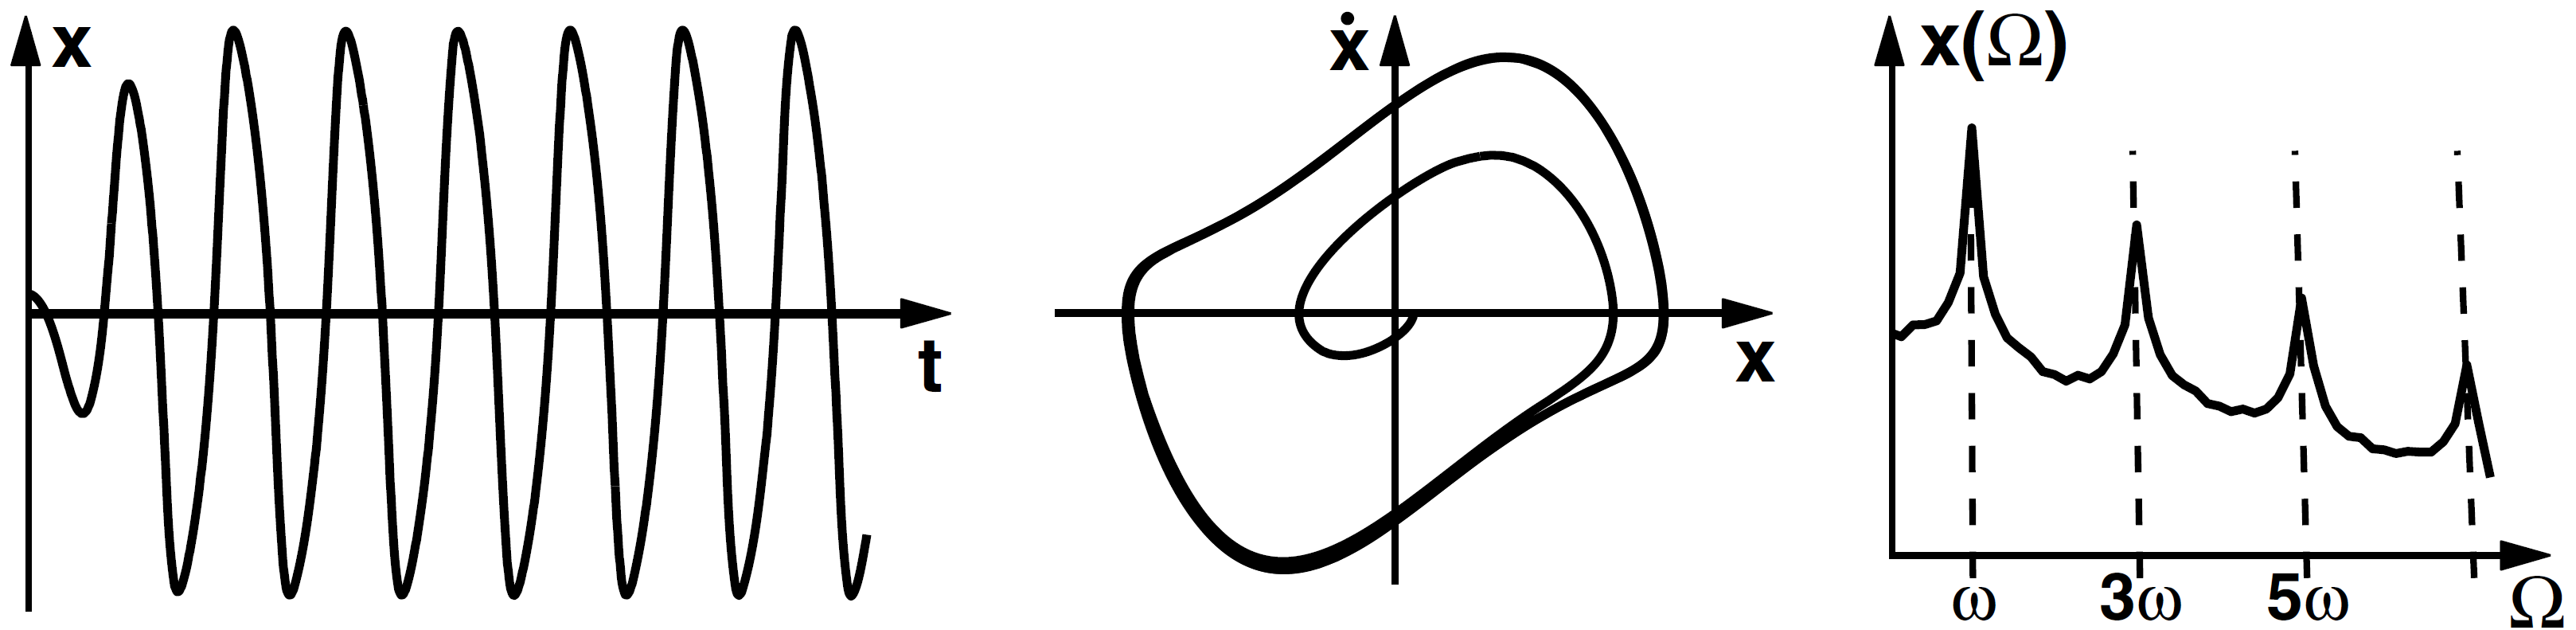
\includegraphics[width=\linewidth]{vdpo.png}
		\caption{The Van-der-Pol oscillator.}
		\label{fig:vdpo}
	\end{subfigure}
	\vline
	\begin{subfigure}{0.45\linewidth}
		\centering
		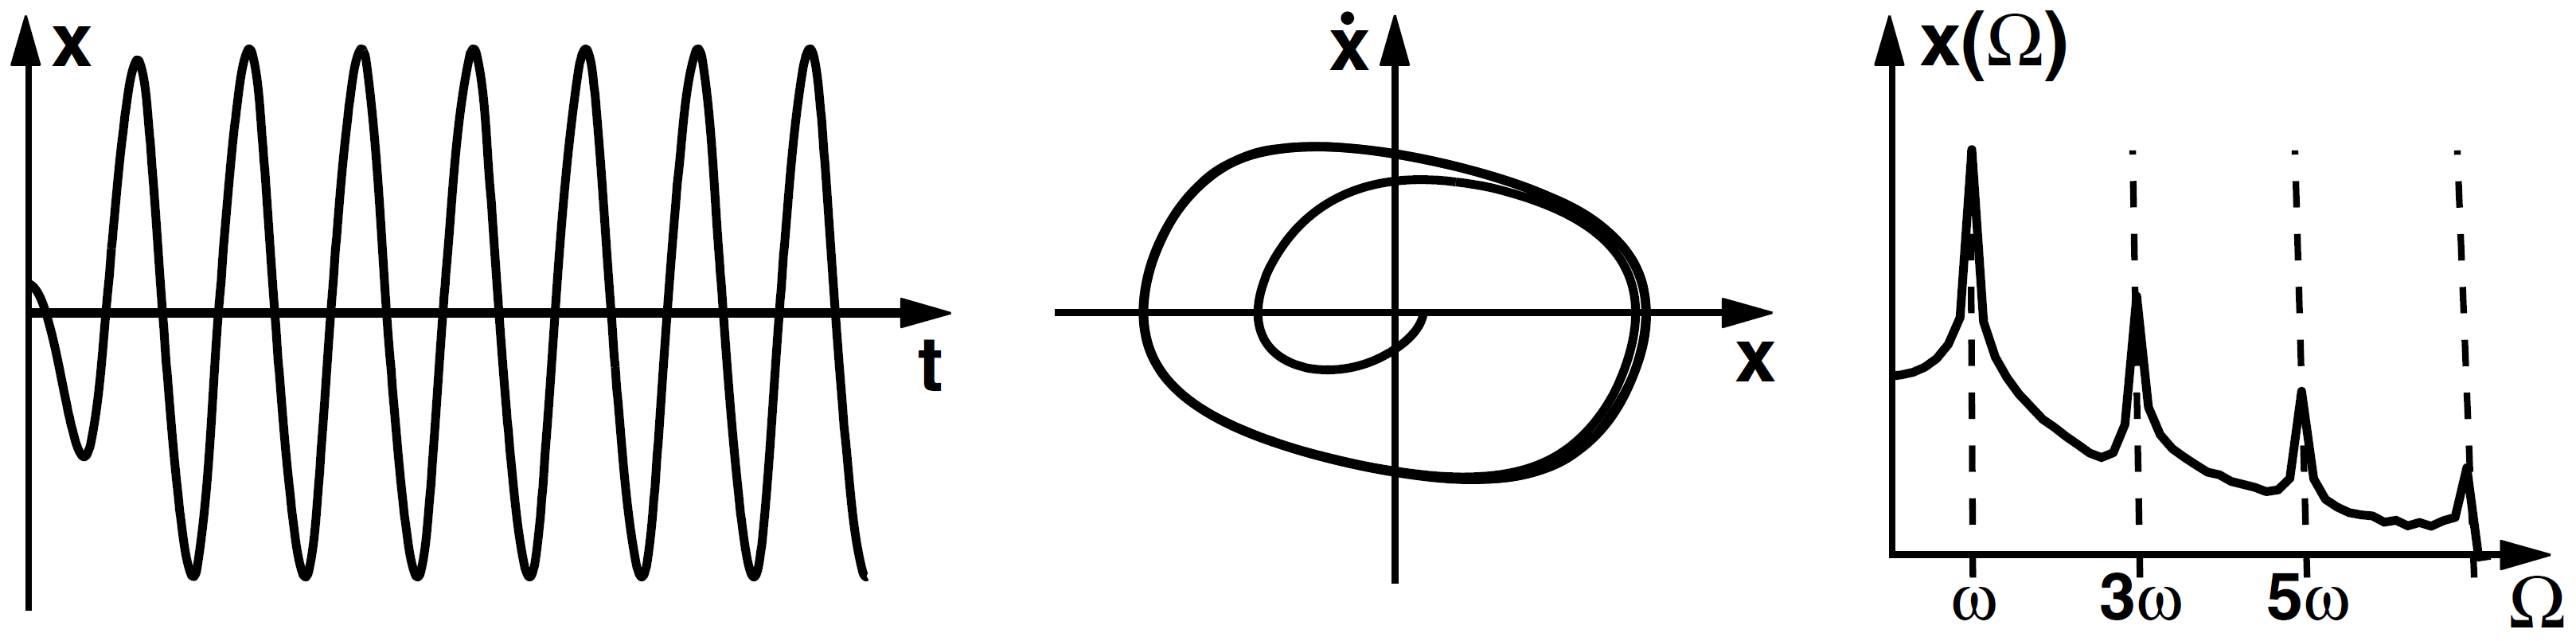
\includegraphics[width=\linewidth]{ro.png}
		\caption{The Rayleigh oscillator}
		\label{fig:ro}
	\end{subfigure}
	\caption{Time series (left), phase space trajectory (middle) and power spectrum (right).}
\end{figure}
\subsection{Rayleigh Oscillator: $N(x,\dot{x})=\dot{x}^3$}
The Rayleigh oscillator is given by
\begin{equation}{\label{eq:ro}}
	\ddot{x}+\gamma\dot{x}+\omega^2+\delta\dot{x}^3=0\quad\rightarrow\quad
	\ddot{x}+(\gamma+\delta\dot{x}^2)\dot{x}+\omega^2x=0
\end{equation}
The damping constant for the Rayleigh oscillator depends on the square of the velocity $\dot{x}^2$.
Arguments similar to those above lead to the conclusion that the Rayleigh oscillator shows sustained oscillations in the parameter range $\gamma<0$ and $\delta>0$.\\
As for the van-der-Pol oscillator, the phase space portrait is almost rectangular but rotated by about $90^\circ$.\\
It can be shown that for the van-der-Pol oscillator the amplitude is independent of frequency and for the Rayleigh it decreases proportional to $\omega^{-2}$.